\documentclass[english]{article}
\usepackage[T1]{fontenc}
\usepackage[utf8]{inputenc}
\setcounter{secnumdepth}{-2}
\setlength{\parindent}{0bp}
\usepackage{xcolor}
\usepackage{calc}
\usepackage{amsmath}
\usepackage{amsthm}
\usepackage{amssymb}
\usepackage{graphicx}

\makeatletter
\theoremstyle{definition}
\newtheorem*{defn*}{\protect\definitionname}
\theoremstyle{plain}
\newtheorem*{lem*}{\protect\lemmaname}
\theoremstyle{plain}
\newtheorem*{thm*}{\protect\theoremname}
\theoremstyle{definition}
\newtheorem*{problem*}{\protect\problemname}
\theoremstyle{definition}
\newtheorem*{sol*}{\protect\solutionname}

\@ifundefined{date}{}{\date{}}
\usepackage{graphicx}
\usepackage{geometry}
\newcommand{\limi}{\underset{n\rightarrow\infty}{\lim}}
\newcommand{\limxz}{\underset{x\rightarrow x_{0}}{\lim}}
\newcommand{\limfxz}{\underset{x\rightarrow x_{0}}{\lim}f(x)}
\newcommand{\limfxm}{\underset{x\rightarrow x_{0}^{-}}{\lim}f(x)}
\newcommand{\limfxp}{\underset{x\rightarrow x_{0}^{+}}{\lim}f(x)}
\newcommand{\limxm}{\underset{x\rightarrow x_{0}^{-}}{\lim}}
\newcommand{\limxp}{\underset{x\rightarrow x_{0}^{+}}{\lim}}
\newcommand{\sqrm}{M_{m\times m}(\mathbb{F})}
\newcommand{\seqa}{(a_{n})_{n=1}^{\infty}}
\newcommand{\seqx}{(x_{n})_{n=1}^{\infty}}
\newcommand{\funcdr}{f:D\rightarrow\mathbb{R}}
\newcommand{\der}{\limxz\frac{f(x)-f(x_{0})}{x-x_{0}}}
\usepackage[all]{pdfprivacy}

\makeatother

\usepackage{babel}
\providecommand{\definitionname}{Definition}
\providecommand{\lemmaname}{Lemma}
\providecommand{\problemname}{Problem}
\providecommand{\solutionname}{Solution}
\providecommand{\theoremname}{Theorem}

\begin{document}
\newgeometry{left=2cm, right=2cm, top=1cm, bottom=2cm}
\title{Introduction to the Cauchy-Schwarz Inequality}

\maketitle
\noindent\fbox{\begin{minipage}[t]{1\columnwidth - 2\fboxsep - 2\fboxrule}%
An introduction to the Cauchy-Schwarz inequality, using some interesting
problems. These questions were taken from a recitation in Linear Algebra
2 at HUJI; all credit belongs to the course staff.%
\end{minipage}}

\medskip{}

\begin{center}
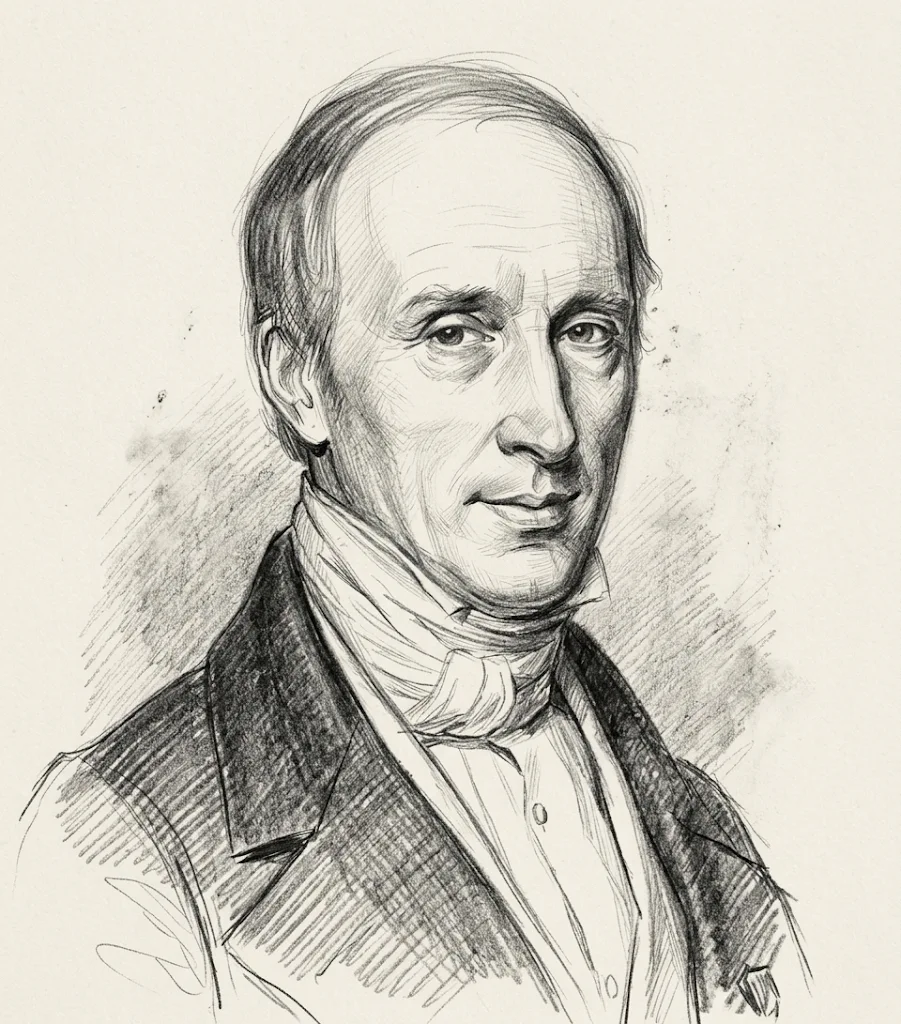
\includegraphics[scale=0.25]{pasted1}
\par\end{center}

We shall first recall some theorems and definitions.

For this page, $\mathbb{F}$ is either $\mathbb{R}$ or $\mathbb{C}$.
\begin{defn*}
inner product

Let $V$ be a vector space over $\mathbb{F}$.

An inner product on $V$ is a function that takes each ordered pair
$\left(u,v\right)$ of elements of $V$ to a number $\left\langle u,v\right\rangle \in\mathbb{F}$
and fulfills the following properties: 

1. positivity on the same vector and definiteness:
\[
\forall v\in V:\left\langle v,v\right\rangle \ge0\text{ and }\left\langle v,v\right\rangle =0\iff v=0
\]

2. additivity in the first slot:
\[
\forall u,v,w\in V:\left\langle u+v,w\right\rangle =\left\langle u,w\right\rangle +\left\langle v,w\right\rangle 
\]
3. homogeneity in the first slot:
\[
\forall u,v\in V,\lambda\in\mathbb{F}:\left\langle \lambda u,v\right\rangle =\lambda\left\langle u,v\right\rangle 
\]

4. conjugate symmetry:
\[
\forall u,v\in V:\left\langle u,v\right\rangle =\overline{\left\langle v,u\right\rangle }
\]
\end{defn*}
\begin{lem*}
basic properties of an inner product

1. Let $v\in V$. Then the function $\varphi:V\rightarrow\mathbb{F}$
defined by $\forall u\in V,\varphi(u)=\left\langle u,v\right\rangle $
is a linear map.

2. 
\[
\forall v\in V:\left\langle 0,v\right\rangle =0\text{ and }\left\langle v,0\right\rangle =0
\]

3.
\[
\forall u,v,w\in V:\left\langle u,v+w\right\rangle =\left\langle u,v\right\rangle +\left\langle u,w\right\rangle 
\]

4. 
\[
\forall\lambda\in\mathbb{F},u,v\in V:\left\langle u,\lambda v\right\rangle =\overline{\lambda}\left\langle u,v\right\rangle 
\]
\end{lem*}
\begin{defn*}
norm, $||v||$

For $v\in V$, the norm of $v$ is 
\[
||v||=\sqrt{\left\langle v,v\right\rangle }
\]
\end{defn*}
\begin{lem*}
for $v\in V,\left\langle v,v\right\rangle \in\mathbb{R}$ and $\left|\left|v\right|\right|\in\mathbb{R}$.
\end{lem*}
\begin{defn*}
dot product

For $x=\left(x_{1},\dots,x_{n}\right),y=\left(y_{1},\dots,y_{n}\right)\in\mathbb{R}^{n}$,
the dot product of $x$ and $y$ is defined by
\[
x\cdot y=\underset{i=1}{\overset{n}{\sum}}x_{i}y_{i}
\]

This is an inner product on $\mathbb{R}^{n}$.
\end{defn*}
\begin{thm*}
The Cauchy-Schwarz Inequality

Let $V$ be an inner product space.

Suppose $u,v\in V$. Then
\[
\left|\left\langle u,v\right\rangle \right|\le||u||\ ||v||
\]

and
\[
\left|\left\langle u,v\right\rangle \right|=||u||\ ||v||\iff u\text{ and }v\text{ are linearly dependent}
\]
\end{thm*}
\begin{problem*}
Let $n\in\mathbb{N}$ and $x_{1},\dots,x_{n}\in\mathbb{R}_{>0}$ such
that $x_{1}+\dots+x_{n}=1$.

Prove that
\[
n^{2}\le\underset{i=1}{\overset{n}{\sum}}\frac{1}{x_{i}}
\]
 
\end{problem*}
\begin{sol*}
\textcolor{teal}{Intuition: in order to solve this problem using the
Cauchy-Schwarz Inequality, we want to choose two vectors $u,v\in\mathbb{R}^{n}$
and an inner product such that the inner product $\left\langle u,v\right\rangle $
gives either the left-hand term or its square root, while their norms
produce terms that help deal with the right-hand side.}

\textcolor{teal}{This is a common method for this type of question.}

\textcolor{teal}{When working in $\mathbb{R}^{n}$, the inner product
will commonly be the standard dot product.}

\textcolor{teal}{Another useful trick is squaring both sides after
applying the inequality.}

\textcolor{teal}{Identifying such vectors and tricks is a matter of
experience. }

\textcolor{teal}{For this question, while one might first try components
with $x_{i}$ directly, trying and adjusting reveals that using square
roots $\sqrt{x_{i}}$ is the key - strengthening the notion that solving
these questions involves some form of trial and error. }
\end{sol*}
\begin{proof}
We can select 
\[
u=\begin{pmatrix}\frac{1}{\sqrt{x_{1}}}\\
\vdots\\
\frac{1}{\sqrt{x_{n}}}
\end{pmatrix},v=\begin{pmatrix}\sqrt{x_{1}}\\
\vdots\\
\sqrt{x_{n}}
\end{pmatrix}
\]

along with the standard dot product which is an inner product in $\mathbb{R}^{n}$.
Therefore, 
\[
\left\langle u,v\right\rangle =\frac{1}{\sqrt{x_{1}}}\cdot\sqrt{x_{1}}+\dots+\frac{1}{\sqrt{x_{n}}}\cdot\sqrt{x_{n}}=\underset{n\text{ times}}{\underbrace{1+\dots+1}}=n
\]

This is well defined since $x_{1},\dots,x_{n}\in\mathbb{R}_{>0}$
(and in particular $n\in\mathbb{N}$ implies $\left|\left\langle u,v\right\rangle \right|=\left\langle u,v\right\rangle $).

Hence, it follows from the Cauchy-Schwarz inequality that
\[
n\le\sqrt{\left\langle u,u\right\rangle }\cdot\sqrt{\left\langle v,v\right\rangle }=\sqrt{\frac{1}{\sqrt{x_{1}}}\cdot\frac{1}{\sqrt{x_{1}}}+\dots+\frac{1}{\sqrt{x_{n}}}\cdot\frac{1}{\sqrt{x_{n}}}}\cdot\sqrt{\sqrt{x_{1}}\cdot\sqrt{x_{1}}+\dots+\sqrt{x_{n}}\cdot\sqrt{x_{n}}}
\]

\[
=\sqrt{\frac{1}{x_{1}}+\dots+\frac{1}{x_{n}}}\cdot\sqrt{x_{1}+\dots+x_{n}}\underset{\text{ since }x_{1}+\dots+x_{n}=1\text{ }}{=}\sqrt{\frac{1}{x_{1}}+\dots+\frac{1}{x_{n}}}\cdot\sqrt{1}=\sqrt{\frac{1}{x_{1}}+\dots+\frac{1}{x_{n}}}
\]

We will now square both sides (they are both non negative) and get
\[
n^{2}\le\frac{1}{x_{1}}+\dots+\frac{1}{x_{n}}
\]
\end{proof}
\begin{problem*}
Let $n\in\mathbb{N}$ and $a_{1},\dots,a_{n}\in\mathbb{R}$. Prove
that
\[
\left(\frac{a_{1}+\dots+a_{n}}{n}\right)^{2}\le\frac{a_{1}^{2}+\dots+a_{n}^{2}}{n}
\]

(taking the root of both sides will give the $AM-QM$ inequality). 
\end{problem*}
\begin{proof}
We can select
\[
u=\begin{pmatrix}a_{1}\\
\vdots\\
a_{n}
\end{pmatrix},v=\begin{pmatrix}\frac{1}{n}\\
\vdots\\
\frac{1}{n}
\end{pmatrix}
\]
along with the standard dot product which is an inner product in $\mathbb{R}^{n}$.
Therefore, 
\[
\left\langle u,v\right\rangle =a_{1}\cdot\frac{1}{n}+\dots+a_{n}\cdot\frac{1}{n}=\frac{a_{1}+\dots+a_{n}}{n}
\]
Hence, it follows from the Cauchy-Schwarz inequality that
\[
\left|\frac{a_{1}+\dots+a_{n}}{n}\right|\le\sqrt{\left\langle u,u\right\rangle }\cdot\sqrt{\left\langle v,v\right\rangle }=\sqrt{a_{1}^{2}+\dots+a_{n}^{2}}\cdot\underset{n\text{ times}}{\underbrace{\sqrt{\frac{1}{n^{2}}+\dots+\frac{1}{n^{2}}}}}=\sqrt{a_{1}^{2}+\dots+a_{n}^{2}}\cdot\sqrt{\frac{n}{n^{2}}}=\sqrt{a_{1}^{2}+\dots+a_{n}^{2}}\cdot\sqrt{\frac{1}{n}}
\]
\[
\therefore\quad\left|\frac{a_{1}+\dots+a_{n}}{n}\right|\le\sqrt{a_{1}^{2}+\dots+a_{n}^{2}}\cdot\sqrt{\frac{1}{n}}
\]
We will now square both sides (they are both non negative) and get
\[
\left(\frac{a_{1}+\dots+a_{n}}{n}\right)^{2}\le\frac{a_{1}^{2}+\dots+a_{n}^{2}}{n}
\]
\end{proof}
\begin{problem*}
Let $V$ be an inner product space over $\mathbb{F}$ and let $0\ne v\in V$.

Prove that $\frac{v}{||v||}$ is the unique element of the unit sphere
of $V$ that is closest to $v$.
\end{problem*}
\begin{quote}
\begin{center}
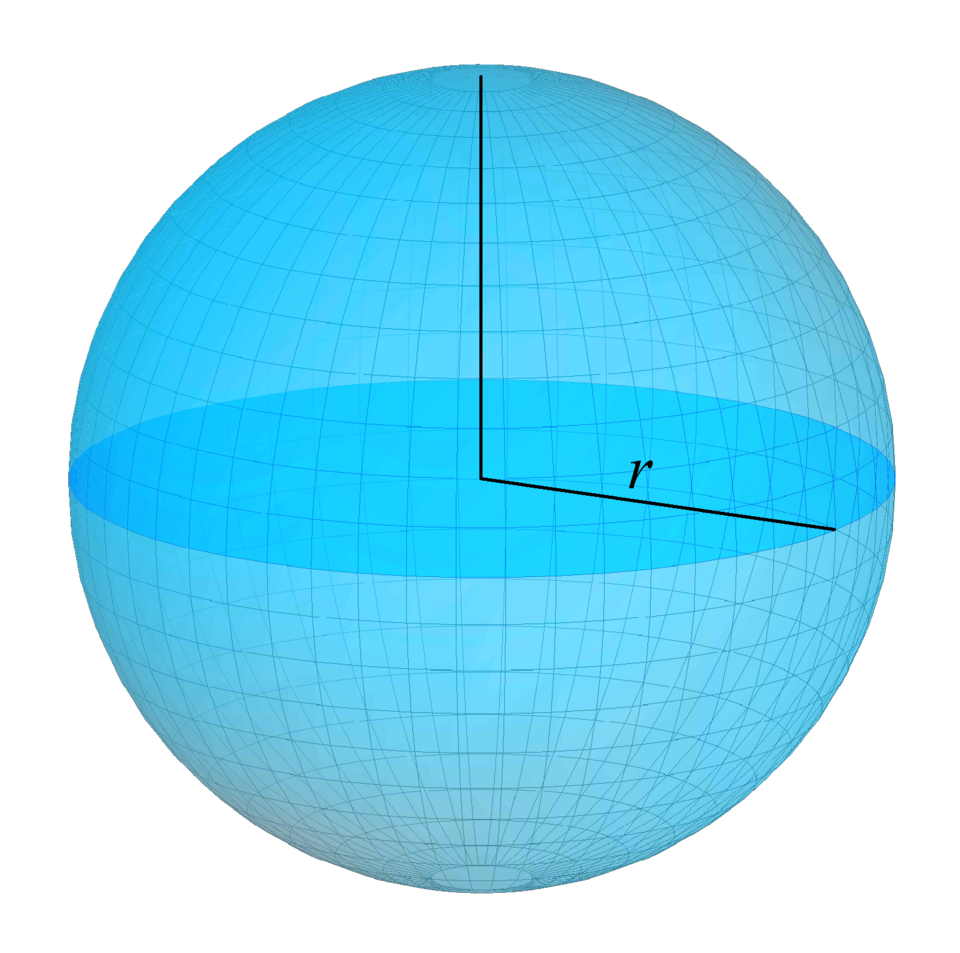
\includegraphics[scale=0.25]{pasted2}
\par\end{center}
\end{quote}
\begin{proof}
Firstly, $\frac{v}{||v||}$ is well defined since $0\ne v$ hence
positivity and definiteness imply $\left\langle v,v\right\rangle >0$
and $||v||=\sqrt{\left\langle v,v\right\rangle }>0$.

Let us recall that the unit sphere of $V$ is 
\[
S_{1}^{V}(0)=\left\{ u\in V:||u||=1\right\} 
\]
Let $u\in S_{1}^{V}(0)$ and we shall inspect the distance between
$u$ and $v$.

\textcolor{violet}{In an inner product space, the distance between
two vectors is defined as the norm of their difference. This measures
the geometric length of the displacement vector connecting one vector
to the other. Since the function $t^{2}$ is strictly increasing on
$[0,\infty)$, looking for the minimum of $||v-u||$ is equivalent
to looking for the minimum of $||v-u||^{2}$.}

\[
||v-u||^{2}=\left(\sqrt{\left\langle v-u,v-u\right\rangle }\right)^{2}=\left\langle v-u,v-u\right\rangle \underset{(*)}{=}\left\langle v,v-u\right\rangle -\left\langle u,v-u\right\rangle 
\]
\[
\underset{\left(**\right)}{=}\left\langle v,v\right\rangle -\left\langle v,u\right\rangle -\left\langle u,v\right\rangle +\left\langle u,u\right\rangle =||v||^{2}+||u||^{2}-\left\langle v,u\right\rangle -\left\langle u,v\right\rangle \underset{\left(***\right)}{=}||v||^{2}+||u||^{2}-\left(\left\langle v,u\right\rangle +\overline{\left\langle v,u\right\rangle }\right)
\]
\[
\underset{u\in S_{1}^{V}(0)}{=}1+||v||^{2}-\left(\left\langle v,u\right\rangle +\overline{\left\langle v,u\right\rangle }\right)\underset{\left(\triangle\right)}{=}1+||v||^{2}-2\text{Re}\left(\left\langle v,u\right\rangle \right)\underset{\text{Re}\left(z\right)\le|z|}{\ge}1+||v||^{2}-2\cdot\left|\left\langle v,u\right\rangle \right|
\]
\[
\underset{\text{Cauchy-Schwarz}}{\ge}1+||v||^{2}-2||u||\ ||v||\underset{u\in S_{1}^{V}(0)}{=}1+||v||^{2}-2\cdot1\cdot||v||=||v||^{2}-2||v||+1=\left(||v||-1\right)^{2}
\]
$(*)$ by additivity and homogeneity in the first slot

$\left(**\right)$ by basic properties of an inner product, parts
3 and 4

$\left(***\right)$ by conjugate symmetry

$\left(\triangle\right)$ $\forall z\in\mathbb{F}:z+\overline{z}=2\text{Re}\left(z\right)$

So the distance squared between a non zero vector $v$ and a vector
on the sphere $u$ is at least $\left(||v||-1\right)^{2}$.

We will now focus on $\frac{v}{||v||}$.

$\frac{v}{||v||}\in S_{1}^{V}(0)$ because 
\[
\left|\left|\frac{v}{||v||}\right|\right|^{2}=\left\langle \frac{v}{||v||},\frac{v}{||v||}\right\rangle =\left\langle \frac{1}{||v||}\cdot v,\frac{1}{||v||}\cdot v\right\rangle \underset{(*)}{=}\frac{1}{||v||}\cdot\left\langle v,\frac{1}{||v||}\cdot v\right\rangle \underset{\left(**\right)}{=}\frac{1}{||v||}\cdot\overline{\frac{1}{||v||}}\cdot\left\langle v,v\right\rangle \underset{\frac{1}{||v||}\in\mathbb{R}}{=}\frac{1}{||v||^{2}}\cdot\left|\left|v\right|\right|^{2}=1
\]

Let us notice that 
\[
\left|\left|v-\frac{v}{||v||}\right|\right|{}^{2}=\left|\left|\left(1-\frac{1}{||v||}\right)v\right|\right|{}^{2}=\left\langle \left(1-\frac{1}{||v||}\right)v,\left(1-\frac{1}{||v||}\right)v\right\rangle \underset{(*)}{=}\left(1-\frac{1}{||v||}\right)\cdot\left\langle v,\left(1-\frac{1}{||v||}\right)v\right\rangle 
\]
\[
\underset{\left(**\right)}{=}\left(1-\frac{1}{||v||}\right)\cdot\overline{\left(1-\frac{1}{||v||}\right)}\cdot\left\langle v,v\right\rangle \underset{1-\frac{1}{||v||}\in\mathbb{R}}{=}\left(1-\frac{1}{||v||}\right)^{2}\cdot\left\langle v,v\right\rangle =\left(1-\frac{1}{||v||}\right)^{2}\cdot||v||^{2}=\left(\left(1-\frac{1}{||v||}\right)||v||\right)^{2}=\left(||v||-1\right)^{2}
\]

Hence, the distance squared between a non zero vector $v$ and a vector
on the unit sphere $u$ is at least the distance squared between $v$
and $\frac{v}{||v||}$, with $\frac{v}{||v||}$ also being on the
unit sphere.

Because distance is non negative, this implies the same for the distance,
and we proved that this element is the closest to $v$.

We will now prove that it's the unique one.

Let $u'\in S_{1}^{V}(0)$ such that $||v-u'||^{2}=\left(||v||-1\right)^{2}$.

We will look at the distance square between $\frac{v}{||v||}$ and
$u'$.

As we showed,

\[
\left|\left|\frac{v}{||v||}-u'\right|\right|^{2}=\left|\left|\frac{v}{||v||}\right|\right|^{2}+||u'||^{2}-\left(\left\langle \frac{v}{||v||},u'\right\rangle +\overline{\left\langle \frac{v}{||v||},u'\right\rangle }\right)\underset{\frac{v}{||v||},u'\in S_{1}^{V}(0)}{=}2-\left(\left\langle \frac{v}{||v||},u'\right\rangle +\overline{\left\langle \frac{v}{||v||},u'\right\rangle }\right)
\]
\[
\underset{\left(\triangle\right)}{=}2-2\text{Re}\left(\left\langle \frac{v}{||v||},u'\right\rangle \right)\underset{\frac{1}{\left|\left|v\right|\right|\in\mathbb{R}}}{=}2-\frac{2}{\left|\left|v\right|\right|}\text{Re}\left(\left\langle v,u'\right\rangle \right)=2-\frac{2}{\left|\left|v\right|\right|}\text{Re}\left(\left\langle v,u'\right\rangle \right)
\]
Furthermore, from $||v-u'||^{2}=\left(||v||-1\right)^{2}$ and what
we showed we get that 
\[
1+||v||^{2}-2\text{Re}\left(\left\langle v,u'\right\rangle \right)=\left(||v||-1\right)^{2}=||v||^{2}-2||v||+1
\]
\[
\therefore\text{Re}\left(\left\langle v,u'\right\rangle \right)=||v||
\]
We will insert this in the last formula and get
\[
2-\frac{2}{\left|\left|v\right|\right|}\text{Re}\left(\left\langle v,u'\right\rangle \right)=2-\frac{2}{\left|\left|v\right|\right|}\cdot||v||=2-2=0
\]

The squared distance is 0, hence $\left\langle \frac{v}{||v||}-u',\frac{v}{||v||}-u'\right\rangle =0$
and by definiteness $\frac{v}{||v||}-u'=0$.

Thus, $u'=\frac{v}{||v||}$ as desired.
\end{proof}

\end{document}
